\documentclass[conference]{IEEEtran}

\IEEEoverridecommandlockouts
\usepackage{cite}
\usepackage{kotex}
\usepackage{float}
\usepackage{amsmath,amssymb,amsfonts}
\usepackage[ruled, vlined]{algorithm2e}
\usepackage{graphicx}
\usepackage{textcomp}
\usepackage{xcolor}
\usepackage{listings}
\usepackage{caption}
\usepackage{subcaption}
\usepackage{multirow}
\usepackage{booktabs}
\usepackage{makecell}
\usepackage{hyperref}
\hypersetup{
    colorlinks=true,
    linkcolor=blue,
    filecolor=magenta,
    urlcolor=cyan,
}
\urlstyle{same}

\lstset{basicstyle=\ttfamily}
\newcommand{\tool}{\textsf{\small JEST}}

\begin{document}

\title{$\textsf{JEST}$: $N\!+\!1$-version Differential Testing of\\
  Both JavaScript Engines and Specification}

\author{
  \IEEEauthorblockN{Jihyeok Park}
  \IEEEauthorblockA{\textit{School of Computing} \\
  \textit{KAIST}\\
  Daejeon, South Korea\\
  jhpark0223@kaist.ac.kr}

  \and

  \IEEEauthorblockN{Seungmin An}
  \IEEEauthorblockA{\textit{School of Computing} \\
  \textit{KAIST}\\
  Daejeon, South Korea\\
  h2oche@kaist.ac.kr}

  \and

  \IEEEauthorblockN{Dongjun Youn}
  \IEEEauthorblockA{\textit{School of Computing} \\
  \textit{KAIST}\\
  Daejeon, South Korea\\
  f52985@kaist.ac.kr}

  \and

  \IEEEauthorblockN{Gyeongwon Kim}
  \IEEEauthorblockA{\textit{School of Computing} \\
  \textit{KAIST}\\
  Daejeon, South Korea\\
  gyeongwon.kim@kaist.ac.kr}

  \and

  \IEEEauthorblockN{Sukyoung Ryu}
  \IEEEauthorblockA{\textit{School of Computing} \\
  \textit{KAIST}\\
  Daejeon, South Korea\\
  sryu.cs@kaist.ac.kr}
}

\maketitle

\begin{abstract}
  Modern programming follows the continuous integration (CI) and continuous
  deployment (CD) approach rather than the traditional waterfall model.  Even
  the development of modern programming languages uses the CI/CD approach to
  swiftly provide new language features and to adapt to new development
  environments.  Unlike in the conventional approach, in the modern CI/CD
  approach, a language specification is no more the oracle of the language semantics
  because both the specification and its implementations (interpreters or compilers) can co-evolve.
  In this setting, both the specification and implementations may have bugs, and
  guaranteeing their correctness is non-trivial.

  In this paper, we propose a novel \textit{$N$+1-version differential testing} to resolve
  the problem.  Unlike the traditional differential testing, our approach
  consists of three steps: 1) to automatically synthesize programs guided by the
  syntax and semantics from a given language specification, 2) to generate
  conformance tests by injecting assertions to the synthesized programs to check their final program
  states, 3) to detect bugs in the specification and implementations via executing
  the conformance tests on multiple implementations, and 4) to localize bugs on
  the specification using statistical information.  We actualize our approach for
  the JavaScript programming language via \( \tool \), which performs
  $N$+1-version differential testing for modern JavaScript engines and ECMAScript,
  the language specification describing the syntax and semantics
  of JavaScript in a natural language.  We evaluated \( \tool \) with four JavaScript engines that
  support all modern JavaScript language features and the latest version of
  ECMAScript (ES11, 2020).  \( \tool \) automatically synthesized 1,700
  programs that covered 97.78\% of syntax and 87.70\% of
  semantics from ES11.  Using the assertion-injected JavaScript programs,
  it detected 44 engine bugs in four different engines and 27
  specification bugs in ES11.
\end{abstract}

\begin{IEEEkeywords}
JavaScript, conformance test generation, mechanized specification,
differential testing
\end{IEEEkeywords}

\section{Artifact Description}

\begin{figure*}
  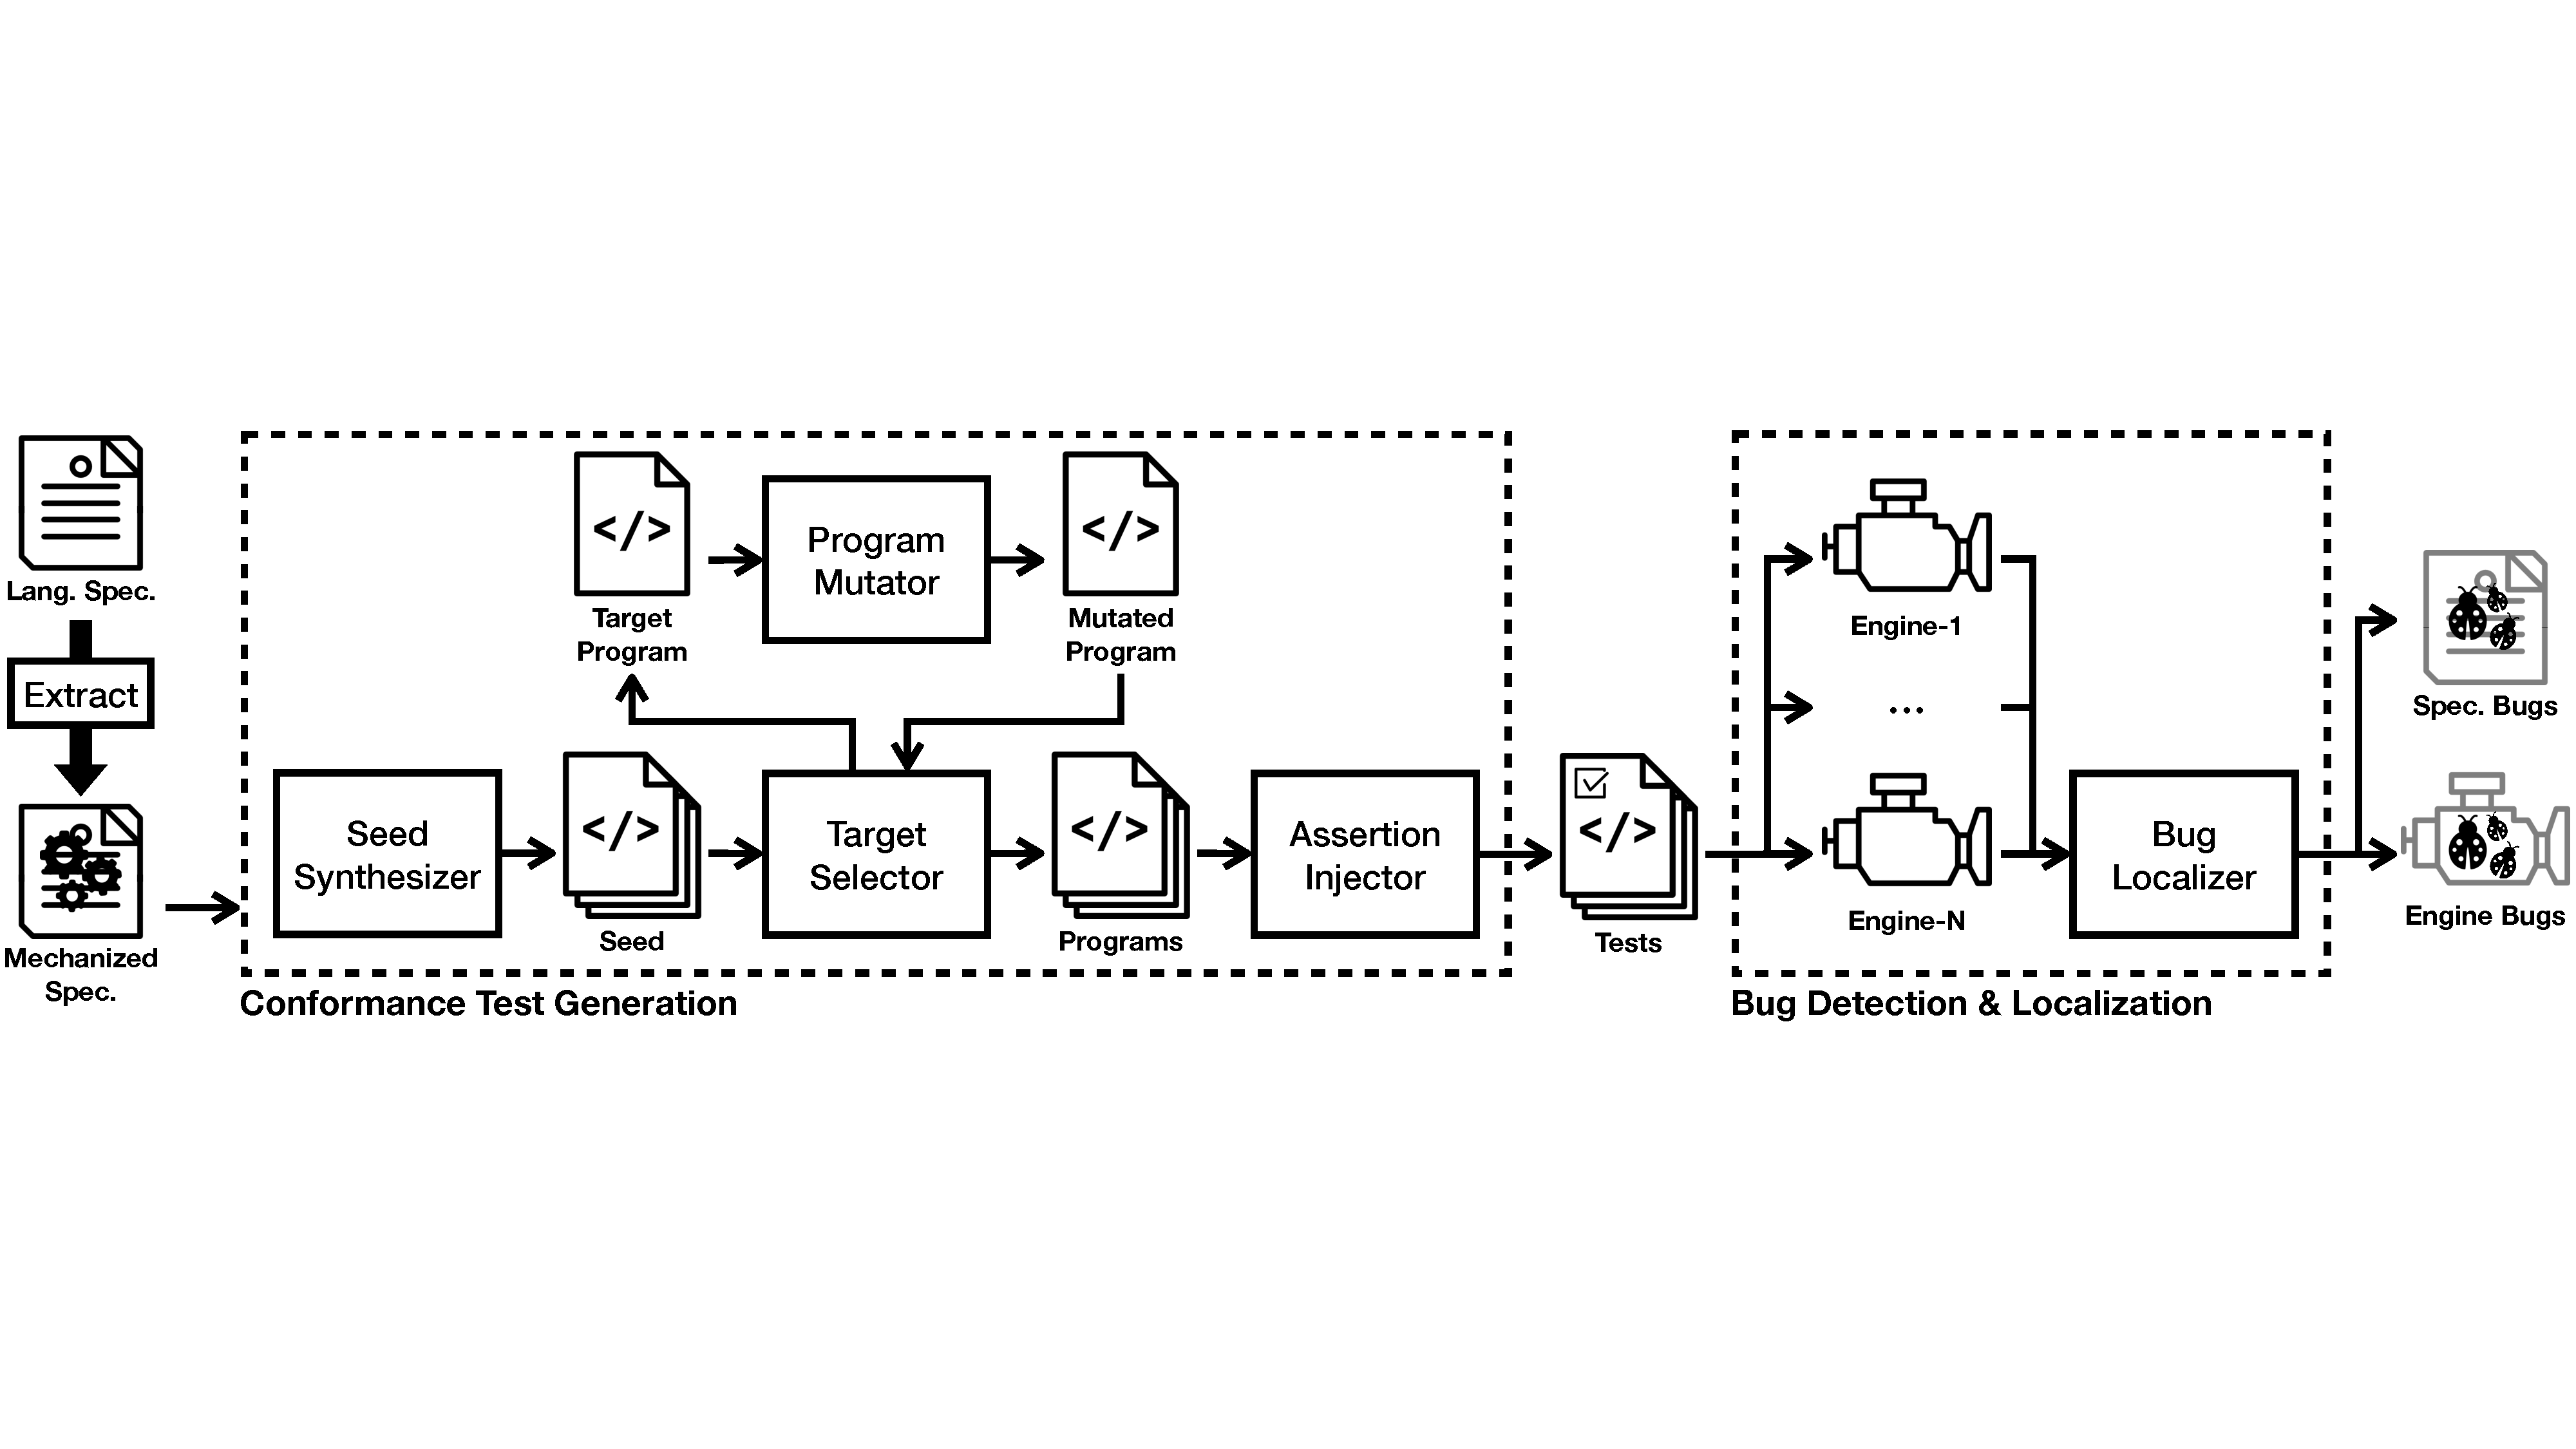
\includegraphics[width=0.98\textwidth]{img/overall.pdf}
  \caption{Overall structure of $N$+1-version differential testing for $N$
    implementations (engines) and one language specification}
  \label{fig:overall}
\end{figure*}

As described in Figure~\ref{fig:overall}, the artifact consists of following
modules to perform $N$+1-version differential testing of JavaScript engines and
specification:
\begin{itemize}
  \item \textbf{SeedSynthesizer} synthesizes an initial seed programs using
    the language syntax.
  \item \textbf{TargetSelector} selects a target program in the program
    pool that potentially increases the coverage of the language semantics by
    the pool.
  \item \textbf{ProgramMutator} generates a new program by mutating a given
    target program in order to increase the coverage of the language semantics
    by the program pool.
  \item \textbf{AssertionInjector} generates conformance tests by injecting
    assertions to the synthesized programs to check their final program states.
  \item \textbf{DifferentialTester} detects bugs in the specification and
    implementations via executing the conformance tests on multiple
    implementations.
  \item \textbf{BugLocalizer} localizes bugs on the specification using
    statistical information.
\end{itemize}


\section{Getting Started Guide}

The artifact is open-source can be obtained by cloning the following git
repository:
\begin{lstlisting}
$ git clone \
  https://github.com/jhnaldo/jest.git
\end{lstlisting}
To build and execute the artifact, you should follow the instrucitons in the
\texttt{INSTALL} file in the artifact.  Since we implement the artifact in
Scala, it requires \texttt{sbt}, which is an intereactive build tool for Scala.
Moreover, for differential testing, you also need to install four different
JavaScript engines: V8 (v8.5), GraalJS (v20.1.0), QuickJS (2020-04-12), and
Moddable XS (v10.3.0).

Additionally, we packaged the artifact in a docker container.  If you want to
skip the environment setting, we recommend you to use it.  You can install the
docker by following the instruction in
\url{https://docs.docker.com/get-started/} and downlaod our docker image with
the following command:
\begin{lstlisting}
$ docker pull jhnaldo/icse-21-jest
$ docker run -it -m=16g --rm \
  jhnaldo/icse-21-jest
# user: guest, password: jest
\end{lstlisting}
\textit{WARNING}: The docker image is 3GB large thus be patient when you
download it and please assign more than 16GB memory for the docker engine.


\section{Basic Commands}

You can run the artifact with the following command:
\begin{lstlisting}
$ jest <sub-command> <option>*
\end{lstlisting}
with the following sub-commands:
\begin{itemize}
  \item \texttt{help} shows the help message.
  \item \texttt{sample} represents \textbf{SeedSynthesizer} and dumps seed
    programs to \texttt{result/seed}.
  \item \texttt{generate} loads seed programs from \texttt{result/seed},
    repeatedly performs \textbf{ProgramMutator} with \textbf{TargetSelector},
    dumps generated programs to \texttt{result/programs}. You can change the
    maximum iteration via the option \texttt{-generate:iter=<number>} (default:
    10).
  \item \texttt{inject} loaded programs from \texttt{result/programs} and dumps
    results of \textbf{AssertionInjector} to the directory \texttt{result/tests}.
  \item \texttt{check} performs \textbf{DifferentialTester} with the tests in
    \texttt{result/tests} and records bugs to \texttt{result/bugs}.
  \item \texttt{localize} performs \textbf{BugLocalizer} for detected bugs in
    the directory \texttt{result/bugs}. When the option
    \texttt{-localize:answer} is given, it reads answers from \texttt{answer}
    and shows their ranks.
  \item \texttt{run} integrates all modules to perform $N$+1-vesion differential
    testing at once.
\end{itemize}
and global options:
\begin{itemize}
  \item \texttt{-time} shows duration time.
  \item \texttt{-bugfix} uses semantics extracted from bug-fixed ECMAScript.
  \item \texttt{-detail} prints intermediate processes.
\end{itemize}


\section{Step-by-Step Instructions}

\subsection{RQ1. Coverage of Generated Tests}

Execute the following command to check the size of seed programs and their
syntactic coverage.
\begin{lstlisting}
$ jest sample
\end{lstlisting}
Then, check the basic program generation wth the following commmand.
\begin{lstlisting}
$ jest generate
\end{lstlisting}
It shows the semantics coverage changes (Figure 4), and the number of generated
programs and covered branches of mutation methods (Table I) during program
generation.  Even though it is impossible to exactly reproduce results because
of the randomness in the program generation, you can check the tendencies by
running the program generation with a large maximum iteration ($\geq 1,000$).
\begin{lstlisting}
$ jest generate -generate:iter=1000
\end{lstlisting}

\subsection{RQ2. Accuracy of Bug Localization}

To reproduce the result in Figure 5, we provide the data used in the evaluation
including programs generated by a single process and example programs invoke
specification/engine bugs we found via the artifact.  Type the following
command:
\begin{lstlisting}
$ rm -r result/programs
$ cp -r data result/programs
$ jest inject && jest check && \
  jest localize -localize:answer
\end{lstlisting}
Moreover, we provide detailed data of each bug detected by the artifact in
\texttt{bugs.md}. You can check the table in Section IV.B with this file.

\subsection{RQ3/4. Bug Detection in JavaScript Engines/Specification}

The file \texttt{bugs.md} also explains the Table II and Table III.

\end{document}
